\documentclass[10pt]{article}
\usepackage[pdftex]{graphicx}
\graphicspath{{./images/}}
\usepackage{amsmath,amssymb}
\usepackage{dirtytalk}
\usepackage{anyfontsize}
\usepackage{xcolor}
\usepackage{hyperref}
\hypersetup{
	colorlinks,
	linkcolor={red!50!black},
	citecolor={blue!50!black},
	urlcolor={blue!80!black}
}
\usepackage[skip=10pt plus1pt, indent=40pt]{parskip}
\usepackage{../../common_styles/csagh}


\begin{document}
	\begin{opening}
		\title{Entregable 4 - PIA}
		\author[Universidad Autónoma de Nuevo León, San Nicolás de los Garza, aldo.hernandezt@uanl.edu.mx]{Aldo Hernández}
		\author[Universidad Autónoma de Nuevo León, San Nicolás de los Garza, abraham.lopezg@uanl.edu.mx]{Abraham López}
		\author[Universidad Autónoma de Nuevo León, San Nicolás de los Garza, gilberto.garciam@uanl.edu.mx]{Damián García}
		\author[Universidad Autónoma de Nuevo León, San Nicolás de los Garza, cristian.antoniosnt@uanl.edu.mx]{Cristian Antonio}
		
		\keywords{...}
		\begin{abstract}			
			Este documento presenta un análisis de las mejoras realizadas a un modelo de Reconocimiento Óptico de Caracteres (OCR) diseñado para transcribir texto de imágenes. El modelo inicial mostró un rendimiento deficiente con valores de pérdida estancados, lo que motivó una revisión integral. Las modificaciones clave incluyeron: mejora en la carga de datos usando pandas y TensorFlow para un mejor control; vectorización de etiquetas mejorada con tokens de máscara y padding adecuados; creación de una clase personalizada CTCOCRModel con implementación optimizada de pérdida CTC; ajustes arquitectónicos para prevenir problemas de longitud de secuencia; refinamientos a la métrica CWERMetric usando \textit{tf.nn.ctc\_greedy\_decoder}; y un mejor cálculo del número de clases utilizando el tamaño del vocabulario de caracteres. Estos cambios resultaron en mejoras significativas del rendimiento, reduciendo la pérdida de validación de 727.3027 a 5.26555, aunque la Tasa de Error de Caracteres (CER) permanece en 1.2292, indicando margen para mejoras adicionales. El documento incluye métricas de rendimiento, gráficos de pérdida y ejemplos de predicciones que demuestran el progreso, reconociendo a la vez la necesidad de mejoras adicionales en trabajos subsecuentes.
		\end{abstract}
		
		\keywords{python, OCR, CNN, TensorFlow, CER}
	\end{opening}
	
	\section{Introducción}
	En este entregable se analizarán los diferentes cambios realizados al modelo de reconocimiento óptico de caracteres (OCR, por sus siglas en inglés), cuyo propósito principal es transcribir texto presente en imágenes de manera precisa y eficiente. Este tipo de modelo es fundamental en aplicaciones como la digitalización de documentos, lectura automatizada de matrículas vehiculares, o extracción de datos de formularios escaneados. Debido al muy bajo rendimiento que ofreció nuestro primer modelo a como esperábamos que funcionara, nos motivó a la revisión y mejora de distintos componentes del mismo.
	
	El objetivo principal de los cambios implementados ha sido reducir la pérdida total del modelo durante el entrenamiento, ya que anteriormente se mantenía en un valor fijo, esto se traduce en una mayor precisión en el reconocimiento de caracteres. Para lograr esto, se abordaron distintos aspectos tanto del preprocesamiento de los datos como de la arquitectura del modelo y el tratamiento de las etiquetas. El análisis presentado en este reporte se enfocará en evaluar el impacto de cada uno de estos cambios en el desempeño global del sistema.
	
	Cada uno de estos cambios será analizado en detalle en las siguientes secciones del entregable, donde se presentarán métricas comparativas entre el modelo antiguo y la versión actualizada. Se incluirán gráficos de pérdida y precisión, además, a partir de estos resultados se discutirá el impacto de las modificaciones implementadas y se propondrán posibles mejoras futuras.
	
	\section{Ajustes principales}
	Para comenzar, cambiamos la manera en cómo se cargan y procesan los datos. Anteriormente se usaba directamente la función \textit{make\_csv\_dataset} del framework TensorFlow para cargar el archivo csv, pero ahora se optó por hacerlo de una forma más controlada. Primero se leen los metadatos del archivo csv (como nombres de archivo y etiquetas) con \textit{pandas.read\_csv} y posteriormente se crea nuestro dataset \textit{tf.data.Dataset} con la función \textit{from\_tensor\_slices} con la finalidad de tener una mayor flexibilidad y control sobre los datos antes de introducirlos al flujo de TensorFlow, esto además permitió el cálculo de cosas como la longitud máxima de etiquetas y el vocabulario de etiquetas de manera más directa sin hacer que TensorFlow se encargue de todo, lo que alentaba todo el proceso.
	
	El siguiente cambio importante fue el cómo se vectorizaban las etiquetas y cómo se les hacía el \textit{padding}. En el modelo anterior el vectorizador se creaba sin un \textit{mask\_token} y se usaba el padding con $99$, esto causaba que este número podría entrar en conflicto con los índices reales de los caracteres y por consecuencia se afectaba a la función de pérdida \textbf{CTC} que es muy sensible a este tipo de detalles. Ahora el vectorizador \textit{char\_to\_num\_global} se inicializa con un \textit{mask\_token} igual a una cadena vacía y un \textit{oov\_token} con valor \textit{"[UNK]"} para hacerlo más robusto frente a vacíos o caracteres no conocidos. Para el \textit{padding} se utilizó un valor de $-1$ ya que es más seguro al estar fuera del rango válido de caracteres. Aun más, nos cercioramos de que las etiquetas y el \textit{padding} sean del tipo \textit{tf.int32} para que la función \textit{ctc\_loss} funcione como se desea.
	
	Al momento de entrenar, antes se utilizaba \textit{keras.Sequential} junto con \textit{model.fit} y la \textbf{pérdida CTC} de Keras, esto no dejaba mucho margen para configurar otros detalles importantes; es por esto que se creó la clase \textbf{CTCOCRModel} que hereda de \textit{keras.Model} y se personalizaron los métodos \textit{train\_step} y \textit{test\_step}. Se hizo este cambio de clase porque buscamos llamar directamente a \textit{tf.nn.ctc\_loss} para definir parámetros concretos como \textit{blank\_index} con un valor de $-1$ porque este número indica qué índice representa el carácter en blanco que necesita la función CTC y si no está bien configurado, el modelo simplemente no aprenderá.
	
	En cuanto a la arquitectura, un ajuste esencial fue en la parte final de la red neuronal, concretamente en cómo se calcula la longitud de la salida de la CNN para la CTC. Antes, la capa de \textit{Reshape} usaba un \textit{img\_width // $4$} pero esto a veces hacía que la secuencia de predicción fuera más corta que la etiqueta real, lo cual rompía la función de \textbf{pérdida CTC}. Para corregir este problema, cambiamos una de las capas de \textit{MaxPooling2D} para que hiciera un menor \textit{downsampling} en la dimensión del ancho junto con \textit{img\_width // $2$} para la longitud de salida. Además, se colocó una verificación explícita que lanza un error si alguna etiqueta es más larga que dicha salida para asegurarnos de que todo esté bien antes de entrenar.
	
	Sobre las métricas, se hicieron ajustes a la métrica \textbf{CWERMetric} ya que antes usaba \textit{keras.ops.nn.ctc\_decode} y se hacía un slicing de las predicciones. Esto generaba que a veces se truncaban los resultados si no estaban bien alineados con la longitud real, en cambio, ahora se usa directamente \textit{tf.nn.ctc\_greedy\_decoder} para una mayor estabilidad. A su vez se mejoró el manejo de SparseTensor y sus tipos de datos para que todo sea compatible con las etiquetas reales.
	
	Finalmente, se cambió cómo se calcula el número total de clases representado por \textit{num\_classes} para la salida del modelo. Antes solamente se usaba la longitud del \textit{set} de caracteres mas uno para el caracter en blanco, pero ahora se utiliza \textit{char\_to\_num\_global.vocabulary\_size() $+ 1$}. Esto ha demostrado ser mejor porque ahora \textit{StringLookup} puede añadir tokens especiales como lo son el \textit{mask\_token} o el \textit{oov\_token} y sin ellos el modelo podría tener un desajuste entre las etiquetas, la salida de la red y la pérdida.
	
	\section{Evaluación del modelo}
	
	Se obtuvieron resultados significativamente superiores al utilizar el modelo actual en comparación con el modelo anterior, como se muestra en la tabla \ref{model_comp}. Esta mejora en el rendimiento puede atribuirse a varios factores, entre ellos una arquitectura optimizada, un mejor ajuste de los hiperparámetros y un entrenamiento más prolongado. Tal como era de esperarse, al incrementar tanto el número de épocas como el tamaño del \textit{batch}, el modelo fue capaz de aprender de manera más eficiente a partir de los datos, lo que se tradujo en un desempeño sustancialmente mejor.
	
	El incremento en las épocas permitió al modelo realizar un mayor número de iteraciones sobre el conjunto de datos, facilitando una convergencia más estable y precisa. Estos diferentes factores contribuyeron a una mejora global en los resultados obtenidos.
	
	No obstante, estos hallazgos se desarrollarán con mayor profundidad en la siguiente sección, donde se presentarán y analizarán en detalle las métricas específicas y los gráficos que evidencian la evolución del rendimiento del modelo a lo largo del entrenamiento.
	
	\begin{table}[!ht]
		\centering
		\caption{Comparación entre modelos}
		\label{model_comp}
		\begin{tabular}{|c|c|c|}
			\hline
			Modelo & Anterior & Actual \\
			\hline
			Epochs & 100 & 100 \\
			\hline
			Learning rate & 0.0010 & 0.0010 \\
			\hline
			Batch size & 1024 & 1024 \\
			\hline
			val\_loss & 727.3027 & 5.26555 \\
			\hline
			CER & N/A & 1.2292 \\
			\hline
		\end{tabular}
	\end{table}
	
	\section{Visualización}
	Recordando los resultados del primer modelo, a pesar de un entrenamiento con ??? épocas se obtuvo una pérdida (\textit{val\_loss}) casi constante de $727$ a lo largo de todo el proceso. Podemos ver el impacto que generaron los ajustes que realizamos durante esta semana en las figuras \ref{fig:loss} y \ref{fig:metrics}. Si bien hemos reducido notablemente la pérdida (de $727$ a $7$), el \textit{Character Error Rate} \textbf{CER} sigue siendo bastante alto y es por eso que el valor no se muestra en la figura \ref{fig:loss}.
	
	\begin{figure}[h]
		\centering
		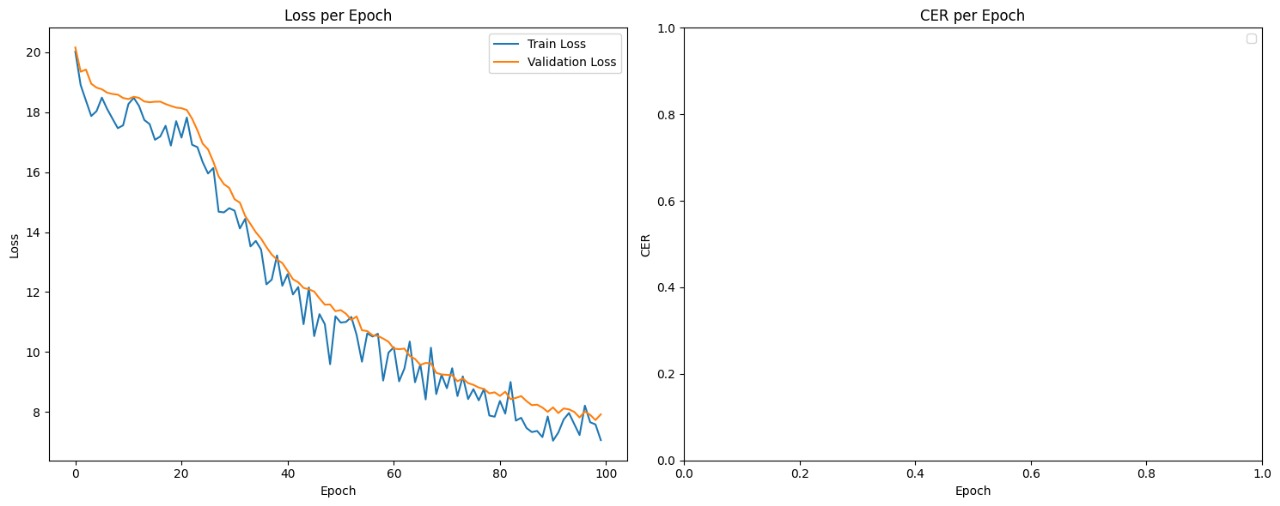
\includegraphics[width=\linewidth]{./images/loss_per_epoch.jpg}
		\caption{Pérdida por época y CER por época.}
		\label{fig:loss}
	\end{figure}
	
	\begin{figure}[h]
		\centering
		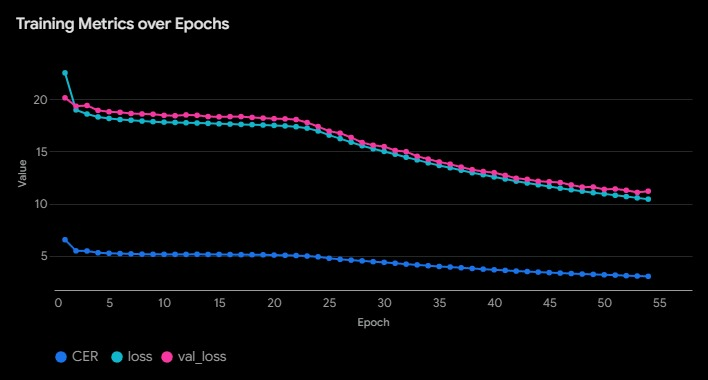
\includegraphics[width=\linewidth]{./images/metrics_over_epoch.jpg}
		\caption{Valor de métricas sobre épocas.}
		\label{fig:metrics}
	\end{figure}
	
	Ya por último podemos ver algunas de las predicciones que hizo nuestro modelo en la figura \ref{fig:pred}. Observamos que el modelo todavía está lejos de tener predicciones acertadas pero con los cambios que realizaremos para la siguiente semana esperamos mejorar eso.
	
	\begin{figure}[!h]
		\centering
		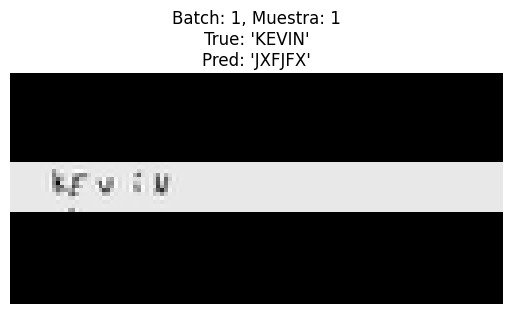
\includegraphics[width=60mm]{./images/prediction1.jpg}
		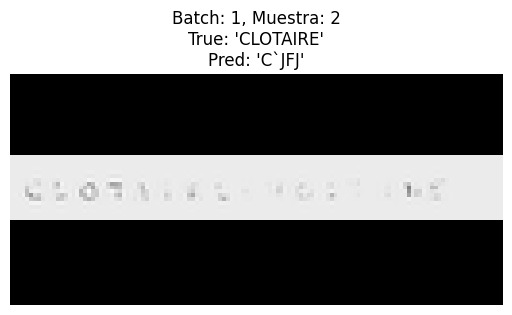
\includegraphics[width=60mm]{./images/prediction2.jpg}
		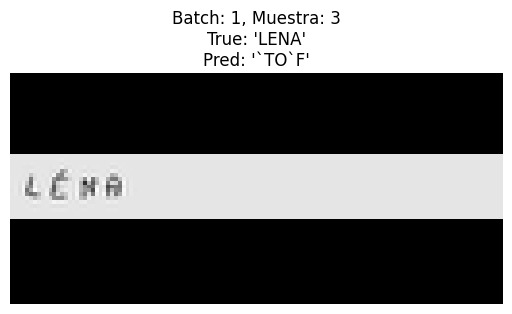
\includegraphics[width=60mm]{./images/prediction3.jpg}
		\caption{Predicción de KEVIN, CLOTAIRE y LENA, respectivamente.}
		\label{fig:pred}
	\end{figure}
	
\end{document}